%UNIT 12: EIGENTHEORY APPLIED TO LINEAR SYSTEMS
%%%%%%%%%%%%%%%%%%%%%%%%%%%
%%%% Put the following at the top of each .tex file  %
\pagestyle{fancy}
\renewcommand{\theUnit}{12}
\ifthenelse{\isundefined{\UnitPageNumbers}}{}{\setcounter{page}{1}}
\rhead{Unit \theUnit: Eigentheory Applied to Linear Systems}
\lhead{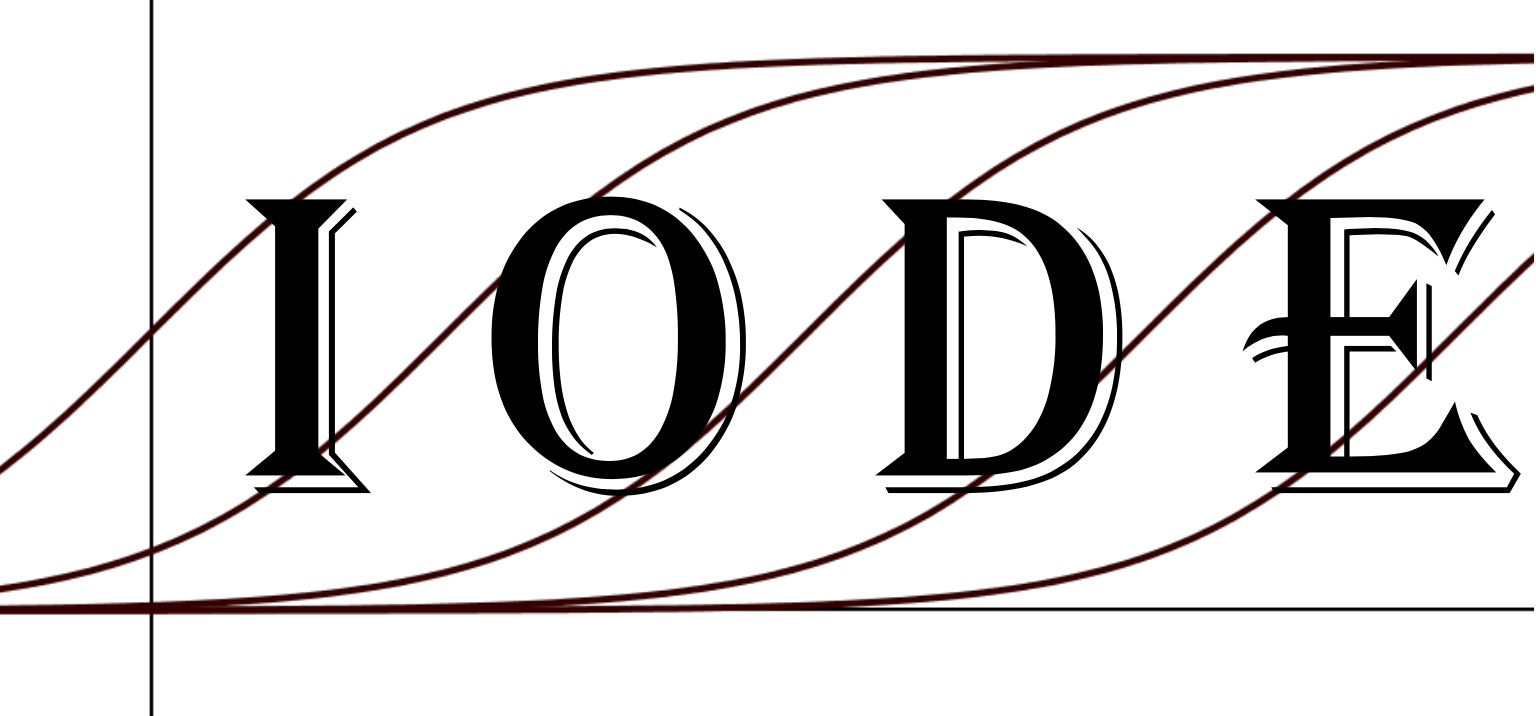
\includegraphics[width=1.25cm]{IODE-logo.png}}
\rfoot{\mypage}
\lfoot{}
\cfoot{}
\fancypagestyle{firstfooter}{\footskip = 50pt}
\renewcommand{\footrulewidth}{.4pt}
%%%%%%%%%%%%%%%%%%%%%%%%%%%
\vspace*{-20pt} \thispagestyle{firstfooter}
\pagebegin{Equilibrium Solutions for Linear Systems}
\begin{align*}\begin{split}
\frac{dx}{dt}&=ax+by\\ \frac{dy}{dt}&= cx+dy
\end{split}\end{align*}

\begin{enumerate}
\item	For each part below, use two different ways (one algebraic and one geometric using nullclines) to figure out the number and location of equilibrium solutions. \label{12problem1}

\begin{enumerate}
\item $\displaystyle
\begin{aligned}
\frac{dx}{dt}&=3x+2y \\
\frac{dy}{dt}&= -2y
\end{aligned}$

\item $\displaystyle
\begin{aligned}
\frac{dx}{dt}&=4x-2y \\
\frac{dy}{dt}&= -2x+y
\end{aligned}$
\end{enumerate}

\item	\label{12problem2} Is it possible to find values of $a, b, c, d$ such that the system of differential equations
\begin{align*}
\frac{dx}{dt}&=ax+by \\
\frac{dy}{dt}&= cx+dy
\end{align*} has \underline{exactly} two equilibrium solutions? Explain why or why not. \vfill

\item \label{12problem3} Develop criteria (in terms of the parameters $a, b, c$, and $d$) that tell us about the number and location of equilibrium solutions for systems of differential equations of the form
\begin{align*}\begin{split}
\frac{dx}{dt}&=ax+by \\
\frac{dy}{dt}&= cx+dy
\end{split}.\end{align*}
\vfill
\end{enumerate}

\clearpage
\pagebegin{Matrix Notation and Equilibrium Solutions for Linear Systems}
\begin{align*}\begin{split}
\frac{dx}{dt}&=ax+by\\ \frac{dy}{dt}&= cx+dy
\end{split}\end{align*}

One way to approach problem \ref{12problem3} is to think about there being an infinite number of equilibrium solutions when the two nullclines coincide. That is, when the equations  $\displaystyle
\begin{aligned}
0&=ax+by\\ 0&= cx+dy
\end{aligned}$ determine the same set of points. Put another way, the equations are \textit{dependent} when $\displaystyle y=-\frac{a}{b}x$ and $\displaystyle y=-\frac{c}{d}x$  are the same equation. Thus, $\displaystyle -\frac{a}{b}=-\frac{c}{d}$, which says that $-ad = -cb$. Rewriting this yields  $ad - bc = 0$.  

As shown next, another way to arrive at this result is to use matrix notation and the fact that two equations are dependent when the determinant of the matrix is zero. 

\[
\begin{matrix} ax+by &=0\\ cx+dy &=0 \end{matrix} 
\Longrightarrow \begin{pmatrix}a&b\\c&d\end{pmatrix}\begin{pmatrix}x\\y\end{pmatrix}=\begin{pmatrix}0\\0\end{pmatrix}
\]

Thus, the equations $ \begin{matrix} ax+by &=0\\ cx+dy &=0 \end{matrix}$ are dependent when the determinant of the coefficient matrix $\begin{pmatrix} a&b \\ c&d \end{pmatrix}$ is zero. That is, when $ad-bc=0$. \\ 

Next, we develop an approach for finding the general solution to a system of differential equations of the form $ \begin{matrix} \frac{dx}{dt}&=ax+by \\\frac{dy}{dt}&= cx+dy  \end{matrix}$  by first finding the value of the exponent (that is, the \textbf{eigenvalue}) associated with any straight line solution \textit{before} finding the slope of the straight line solutions (typically called \textbf{eigensolutions}). Note that in your previous work you first found the slope of straight line solutions and then found the exponent. Some students have referred to this as the ``slope first'' method. In the pages that follow, an alternative approach is developed: the ``eigenvalue first'' method. \\ 

We develop this alternative method for four reasons:
\begin{itemize}
\item	The eigenvalue first method can be used for systems of three or more differential equations whereas the slope first method cannot.
\item	Oftentimes just knowing the eigenvalues is sufficient for understanding the overall picture of solutions in the phase plane and so therefore this method is more efficient.
\item	The eigenvalue first approach makes important connections with linear algebra.
\item	The eigenvalue first approach is algebraically more efficient.
\end{itemize}

\clearpage

%%%%%%%%%%%%%%%%%%%%%%%%%%
\pagebegin{Eigenvalue First Method}

For linear systems of the form  $ \begin{matrix} \frac{dx}{dt}&=&ax+by \\\frac{dy}{dt}&=& cx+dy  \end{matrix}$, one way to determine the exponent (i.e. $\lambda$, the eigenvalue) for possible straight line solutions (or eigensolutions) is to use the fact that if eigensolutions exist in the phase plane, then  $\frac{dx}{dt}=\lambda x$ and  $\frac{dy}{dt}=\lambda y$.  

\begin{enumerate}[resume]
\item	Explain why this has to be true. \label{12problem4}
\vspace{2in}
\end{enumerate}

Combining the fact that $ \begin{matrix} \frac{dx}{dt}&=&ax+by \\\frac{dy}{dt}&=& cx+dy  \end{matrix}$  with the fact that for straight line solutions   $\frac{dx}{dt}=\lambda x$ and $\frac{dy}{dt}=\lambda y$ along the straight line, we can set up the following two equations:  
\begin{equation}
\begin{matrix} ax+by &=\lambda x\\ cx+dy &=\lambda y \end{matrix} \tag{1}\label{eq:1}
\end{equation}
Rearranging these equations we get  
\begin{equation}
 \begin{matrix} (a-\lambda)x+by &=0\\ cx+(d-\lambda)y &=0 \end{matrix} \tag{2}\label{eq:2}
\end{equation}
Note that although these equations look similar to the nullcline equations, the coefficients are different. \\

If the equations from \eqref{eq:2} are dependent then you get straight line solutions with a particular value of $\lambda$ corresponding to an exponent from the straight line solution.
\begin{enumerate}[resume]
\item Explain why this has to be true. \label{12problem5}
\end{enumerate}
\clearpage

Rewriting these dependent equations in slope form yields  $y=-\frac{a-\lambda}{b}x$ and $y=-\frac{c}{d-\lambda}x$  
and thus $-\frac{a-\lambda}{b}=-\frac{c}{d-\lambda}$  .  Rearranging this last equation we get the following:
\begin{align*}
&(a-\lambda)(d-\lambda)-bc=0\\ 
\Rightarrow& \lambda^2-(a+d)\lambda+(ad-bc)=0\\
\Rightarrow& \lambda=\frac{(a+d)\pm \sqrt[]{(a+d)^2-4(ad-bc)}}{2}
\end{align*}
             

We can more efficiently obtain this same result using matrix notation and the fact that two equations are dependent when the determinant of the coefficient matrix is zero as follows:

\[ \begin{matrix}
(a-\lambda)+by &=0\\ cx+(d-\lambda)y &=0 \end{matrix}
\Longrightarrow \begin{pmatrix}
a-\lambda &b\\ c& d-\lambda
\end{pmatrix}\begin{pmatrix}x\\y\end{pmatrix} = \begin{pmatrix}
0\\0
\end{pmatrix}\]

Thus, the equations $\begin{matrix}
(a-\lambda)+by &=0\\ cx+(d-\lambda)y &=0 \end{matrix}$  are dependent when the determinant of the coefficient matrix  \[\begin{pmatrix}
a-\lambda &b\\ c& d-\lambda
\end{pmatrix}\] is zero. That is, when  $(a-\lambda)(d-\lambda)-bc=0$. 

\textbf{EXAMPLE:}
\begin{quote}
Determine the general solution for the system of differential equations 
\[\begin{matrix} \frac{dx}{dt}&=&4x+2y \\\frac{dy}{dt}&=& x+3y  \end{matrix}
\]using the ``eigenvalue first'' approach. 
\end{quote}

In order to get eigensolutions, we need to have 
\begin{align*}
&\begin{matrix} 4x+2y &=& \lambda x \\x+3y  &=& \lambda y  \end{matrix}\\
\Rightarrow & \begin{matrix} (4-\lambda)x+2y &=& 0 \\x+(3-\lambda)y  &=& 0 \end{matrix}\\
\Rightarrow	& \begin{pmatrix}
4-\lambda &2\\ 1& 3-\lambda
\end{pmatrix}\begin{pmatrix}x\\y\end{pmatrix} = \begin{pmatrix}
0\\0
\end{pmatrix}\\
\Rightarrow & (4-\lambda)(3-\lambda)-2=0\\
\Rightarrow & \lambda^2-7\lambda+10=0\\
\Rightarrow & (\lambda-5)(\lambda-2)=0\\
\mathbb{} \Rightarrow & \lambda=2, \lambda=5
\end{align*}
           
\underline{For $\lambda = 2$}

Since these two equations $\begin{matrix} 4x+2y &=& 2 x \\x+3y  &=& 2 y  \end{matrix}$ are dependent, we can use either one to determine the straight line of vectors (called eigenvectors) in the phase plane. In this case, straight line solutions are found along the line $y = -x$. 

Any solution along this line can therefore be written as  
\[ \begin{pmatrix}x(t)\\y(t)\end{pmatrix}=k_1e^{2t}\begin{pmatrix}1\\-1\end{pmatrix}.
\]
\underline{For   $\lambda= 5$}

Since these two equations $\begin{matrix} 4x+2y &=& 5 x \\x+3y  &=& 5 y  \end{matrix}$ are dependent, we can use either one to determine the straight line of vectors (called eigenvectors) in the phase plane. In this case, straight line solutions are found along the line  $y=\frac{1}{2}x$.

Any solution along this line can therefore be written as  
\[ \begin{pmatrix}x(t)\\y(t)\end{pmatrix}=k_2e^{5t}\begin{pmatrix}2\\1\end{pmatrix}.
\]


The general solution is therefore
\[
\begin{pmatrix}x(t)\\y(t)\end{pmatrix}=k_1e^{2t}\begin{pmatrix}1\\-1\end{pmatrix}+k_2e^{5t}\begin{pmatrix}2\\1\end{pmatrix}.
\]

\begin{enumerate}[resume]
\item	In the previous example the general solution was determined to be \label{12problem6}
\[
\begin{pmatrix}x(t)\\y(t)\end{pmatrix}=k_1e^{2t}\begin{pmatrix}1\\-1\end{pmatrix}+k_2e^{5t}\begin{pmatrix}2\\1\end{pmatrix}.
\]
What is the specific solution for the initial condition  $(-3, -2)$? Without using technology, sketch the graph of this solution in the phase plane (for $t\to\infty$  and as $t\to-\infty$) and explain how you figured out what the graph looks like based on the equations for the solution.
\end{enumerate}

\clearpage
 
%%%%%%%%%%%%%%%%%%%%%%%%%%%%%%%%%%%%%%%%%%
\pagebegin{Homework Set 12}

\begin{enumerate}
\item	If the general solution for a system of differential equations of the form   
\[ \begin{matrix} \frac{dx}{dt}&=&ax+by \\\frac{dy}{dt}&=& cx+dy  \end{matrix}\] 
is  
\[
\begin{pmatrix}x(t)\\y(t)\end{pmatrix}=k_1e^{-2t}\begin{pmatrix}-1\\4\end{pmatrix}+k_2e^{-t} \begin{pmatrix}2\\1\end{pmatrix},
\]
 what do solutions in phase plane look like? What do solutions that are not straight lines look like? Do they curve a particular way? Figure out a way to use the general solution (without technology) to decide. Explain and graph your ideas.\label{12HWproblem1}

\item	Repeat problem \ref{12HWproblem1} for the general solution \label{12HWproblem2}
\[
\begin{pmatrix}x(t)\\y(t)\end{pmatrix}=k_1e^{- t} \begin{pmatrix}2\\1\end{pmatrix}+k_2e^{3t}\begin{pmatrix}-1\\1\end{pmatrix}.
\]

\item	Repeat problem \ref{12HWproblem1} for the general solution \label{12HWproblem3}
\[
\begin{pmatrix}x(t)\\y(t)\end{pmatrix}=k_1e^{0t}\begin{pmatrix}1\\2\end{pmatrix}+k_2e^{-2t}\begin{pmatrix}-3\\2\end{pmatrix}.
\]

\item	For each of the following systems of differential equations, find the general solution and then sketch the \textbf{phase portrait} (i.e. graphs of solutions viewed in the phase plane) \underline{without} using technology. \label{12HWproblem4}

\begin{enumerate*}

\item $\displaystyle \begin{matrix}\frac{dx}{dt}&=&2x+y\\ \frac{dy}{dt}&=& x+y
\end{matrix}$
\hspace{.5in}
\item $\displaystyle \begin{matrix}\frac{dx}{dt}&=&-4x-2y\\ \frac{dy}{dt}&=& -x-3y
\end{matrix}$
\hspace{.425in}
\item $\displaystyle \begin{matrix}\frac{dx}{dt}&=&4x+2y\\ \frac{dy}{dt}&=& x+3y
\end{matrix}$

\end{enumerate*}

\begin{enumerate*}[resume]

\item $\displaystyle \begin{matrix}\frac{dx}{dt}&=&4x-2y\\ \frac{dy}{dt}&=& -2x+y
\end{matrix}$
\hspace{.4in}
\item $\displaystyle \begin{matrix}\frac{dx}{dt}&=&y\\ \frac{dy}{dt}&=& -4x-y
\end{matrix}$
\hspace{.5in}
\item $\displaystyle \begin{matrix}\frac{dx}{dt}&=&y\\ \frac{dy}{dt}&=& 2x-y
\end{matrix}$

\end{enumerate*}

\begin{enumerate*}[resume]

\item $\displaystyle \begin{matrix}\frac{dx}{dt}&=&2x\\ \frac{dy}{dt}&=& 2y
\end{matrix}$
\hspace{.8in}
\item $\displaystyle \begin{matrix}\frac{dx}{dt}&=&-3x-\frac{1}{2}y\\ \frac{dy}{dt}&=& 6x+y
\end{matrix}$

\end{enumerate*}


\item	For the system of differential equations   \label{12HWproblem5}
\[ \begin{matrix} \frac{dx}{dt}&=&rx+2y \\\frac{dy}{dt}&=& 3x+ry  \end{matrix}\] 
figure out all the possible types of equilibrium solutions for different values of $r$, where $r$ is some real number. Show all work to support your conclusions.


\item	Denise claims that all solutions (except the equilibrium solution) to the system of differential equations  
\[ \begin{matrix} \frac{dx}{dt}&=&ax+by \\\frac{dy}{dt}&=& cx+dy  \end{matrix}\]   will spiral if $(ad-bc)$ is negative. Do you are agree with Denise's claim? If yes, justify your response. If not, explain why not. \label{12HWproblem6}

\item \label{12HWproblem7}
Consider the following system:
\[ \begin{matrix} \frac{dx}{dt}&=&px+qy \\\frac{dy}{dt}&=& cx+dy  \end{matrix}\]
\begin{enumerate}
\item Explain why if the eigenvalues are distinct real numbers, the general form of the solution can be written as
\[
\begin{pmatrix}x(t)\\y(t)\end{pmatrix}=c_1e^{\lambda_1t}\phi_1+c_2 e^{\lambda_2t}\phi_2
\]
where $\phi_1$ and $\phi_2$ are the eigenvectors associated with $\lambda_1$ and $\lambda_2$. \label{12HWproblem7parta}
\item Explain why if the eigenvalues are complex numbers of the form $a \pm bi$ then the general solution is of the form
\[
\begin{pmatrix}x(t)\\y(t)\end{pmatrix}=e^{at}v
\]
where $v$ is a vector containing arbitrary constants $c_1$ and $c_2$ and other terms involving $\sin(t)$ and $\cos(t)$. \label{12HWproblem7partb}
\item Complete the following table by reflecting on and organizing what you've figured out about the phase portrait for systems of linear differential equations based on knowing just the eigenvalues. \label{12HWproblem7partc}
\end{enumerate}

\begin{center}
\renewcommand{\arraystretch}{1.5}
\begin{tabular}{ccc}
\underline{Eigenvalues}	&
\underline{Typical phase portrait}	&
\underline{Basic format of the general solution} \\
two distinct positive \\ real numbers && \\ \hline
one positive and one \\ negative real number && \\ \hline
two distinct negative \\ real numbers && \\ \hline
a complex conjugate pair \\ with negative real part && \\ \hline
a complex conjugate pair \\ with positive real part && \\ \hline
a complex conjugate pair \\ with no real part && \\ \hline
\end{tabular}
\end{center}

\item \label{11HWproblem8}
\begin{enumerate}
\item Go to the glossary and identify all terms that are relevant to this unit and list those terms here.
\item Are there other vocabulary terms that you think are relevant for this unit that were not included? If yes, list them.
\end{enumerate}
\end{enumerate}


